\begin{question}
\noindent On a Valorant esports tournament overlay, a designer plots the positions of two identical map icons, triangle $J$ and triangle $K$, on a coordinate grid to test a mirroring animation effect.

\begin{center}
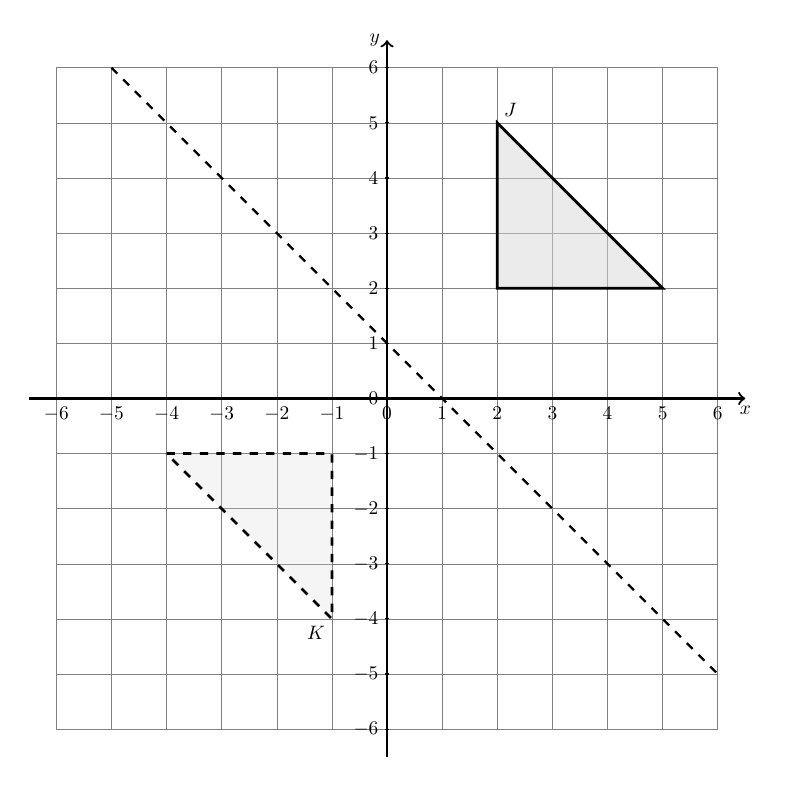
\begin{tikzpicture}[scale=0.7, transform shape]
    % Define colours
    \definecolor{borderColour}{HTML}{000000}
    \definecolor{fillColour}{HTML}{D8D8D8}

    % Define axis scale
    \def\axisLimit{6}

    % Draw grid
    \draw[step=1cm,gray,very thin] (-\axisLimit,-\axisLimit) grid (\axisLimit,\axisLimit);

    % Draw axes
    \draw[thick,->] (-\axisLimit-0.5,0) -- (\axisLimit+0.5,0) node[anchor=north] {$x$};
    \draw[thick,->] (0,-\axisLimit-0.5) -- (0,\axisLimit+0.5) node[anchor=east] {$y$};

    % Label x-axis and y-axis
    \foreach \x in {-\axisLimit,...,\axisLimit}
        \draw (\x cm,1pt) -- (\x cm,-1pt) node[anchor=north] {$\x$};
    \foreach \y in {-\axisLimit,...,\axisLimit}
        \draw (1pt,\y cm) -- (-1pt,\y cm) node[anchor=east] {$\y$};

    % Draw the mirror line y = -x + 1 (i.e. y = 1 - x)
    \draw[thick,dashed] (-5,6) -- (6,-5) node[anchor=south west] {};

    % Define coordinates for triangle J
    \coordinate (A) at (2,5);
    \coordinate (B) at (2,2);
    \coordinate (C) at (5,2);

    % Draw triangle J
    \filldraw[fill=fillColour, draw=borderColour, line width=1pt, fill opacity=0.5] (A) -- (B) -- (C) -- cycle;
    \node[above right] at (A) {$J$};

    % Define coordinates for triangle K (reflection of J in y = -x + 1)
    \coordinate (A') at (-4,-1);
    \coordinate (B') at (-1,-1);
    \coordinate (C') at (-1,-4);

    % Draw triangle K
    \filldraw[fill=fillColour, draw=borderColour, line width=1pt, fill opacity=0.25, dashed] (A') -- (B') -- (C') -- cycle;
    \node[below left] at (C') {$K$};

\end{tikzpicture}
\end{center}

\noindent Triangle $J$ is reflected onto triangle $K$, as shown on the grid.

\noindent Describe fully the single transformation that maps triangle $J$ onto triangle $K$.

\vspace{4cm}

\begin{flushright}
    \answerlines{2}{2}
\end{flushright}
\end{question}